\scanpage{3}

\diagram{\begin{tikzcd}[ampersand replacement=\&,column sep=large,row sep=small]
E_0\arrow[r,bend left=50,"\delta_0"]\&E_1\arrow[l,shift right=1.2ex,"p_0"']\arrow[l,shift left=1.2ex,"p_1"]\arrow[r,bend left=50,"{\delta_1,\delta_2,\delta_3}"]\arrow[r,bend left=60]\arrow[r,bend left=70]\&E_2\arrow[l,shift right=2.2ex,"p_{12}"']\arrow[l,"p_{23}"']\arrow[l,shift left=2.2ex,"p_{13}"]\\
\&\mathcal G_2\arrow[d,phantom,"\in" rotate=90]\&\mathcal G_3\arrow[d,phantom,"\in" rotate=90]\\
\&\sigma\&\overbrace{\rho,\sigma_1,\sigma_2,\sigma_3}\\
\&\&\rho^2
\end{tikzcd}}
\diagram{\deleted{\mbox{\begin{tikzcd}[ampersand replacement=\&,column sep=large]
{}\arrow[r,bend right=40,"\unsure{\delta_1}"']\arrow[r,bend right=55,"\unsure{\delta_2}"']\arrow[r,bend right=70,"\delta_3"']\&{}
\end{tikzcd}}}}
\[\boxed{\begin{aligned}
\delta_3(x,y)&=(x,x,y)\\
\delta_1(x,y)&=(y,x,x)\\
\delta_2(x,y)&=(x,y,x)
\end{aligned}}\]
\margin{\deleted{$\delta_1\sigma(x,y)=(y,y,x)$}\quad $=$\\$\unsure{\sigma|\delta}_3\delta_3$}
\mspage{\textcircled{1}}
\[p_{\unsure{1|0}}=p_0\sigma,\quad p_0=p_1\sigma\]
\[\boxed{\begin{aligned}
p_{12}(x,y,z)&=(x,y)\\
p_{\deleted{\unsure{21}}\inserted{23}}(x,y,z)&=(y,z)\\
p_{31}(x,y,z)&=(z,x)
\end{aligned}}\]
\margin{$\rho(x,y,z)=(y,z,x)$}
\[\deleted{p_{\unsure{12}}=p_{23}}\]
\[\boxed{\left\{\begin{aligned}
p_{23}&=p_{12}\rho\\
p_{31}&=p_{23}\rho=p_{12}\rho^2\\
p_{12}&=p_{31}\rho=p_{23}\rho^2
\end{aligned}\right.}\]
\[\begin{aligned}
\sigma p_{12}&=p_{12}\sigma_3\\
\sigma p_{23}&=p_{23}\sigma_1\\
\sigma p_{31}&=p_{31}\sigma_2
\end{aligned}\]
\[\deleted{(x,y,z)\longrightarrow(y,z,x)\longrightarrow(y,z)}\]
\[\left\{\begin{aligned}
\delta_1&=\rho\delta_2=\rho^2\delta_3\\
\delta_2&=\rho\delta_3=\rho^2\delta_1\\
\delta_3&=\rho\delta_1=\rho^2\delta_2{}^{\unsure{a|\leftarrow}}
\end{aligned}\right.\]

\deleted{\unsure{a}} Il suffit de avoir $p_0,p_{12},\delta_0,\delta_1$ entre les trois ensembles $E_0$, $(E_1,\mathcal G_2)$, $(E_2,\mathcal G_3)$, avec les relations
\[\boxed{p_0\delta_0=\mathrm{id}_{E_0}}\quad\deleted{p_{\unsure{1|12}}\delta_{\unsure{1|0}}}\]
\[\delta_0p_0=p_{12}\underset{\rho^{\deleted{\unsure{2|\sigma}}}\delta_1}{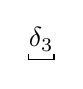
\begin{tikzpicture}[baseline=(term.base)]\node[inner sep=0pt] (term) {$\delta_3$};\draw ([yshift=-1pt]term.south west) -- ([yshift=-3pt]term.south west) -- ([yshift=-3pt]term.south east) -- ([yshift=-1pt]term.south east);\end{tikzpicture}}=\underset{p_{12}\rho}{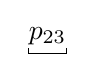
\begin{tikzpicture}[baseline=(term.base)]\node[inner sep=0pt] (term) {$p_{23}$};\draw ([yshift=-1pt]term.south west) -- ([yshift=-3pt]term.south west) -- ([yshift=-3pt]term.south east) -- ([yshift=-1pt]term.south east);\end{tikzpicture}}\underset{\deleted{\unsure{\rho}}}{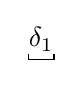
\begin{tikzpicture}[baseline=(term.base)]\node[inner sep=0pt] (term) {$\delta_1$};\draw ([yshift=-1pt]term.south west) -- ([yshift=-3pt]term.south west) -- ([yshift=-3pt]term.south east) -- ([yshift=-1pt]term.south east);\end{tikzpicture}}=\underset{p_{12}\rho^2}{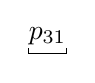
\begin{tikzpicture}[baseline=(term.base)]\node[inner sep=0pt] (term) {$p_{31}$};\draw ([yshift=-1pt]term.south west) -- ([yshift=-3pt]term.south west) -- ([yshift=-3pt]term.south east) -- ([yshift=-1pt]term.south east);\end{tikzpicture}}\underset{\rho^2\delta_1}{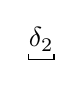
\begin{tikzpicture}[baseline=(term.base)]\node[inner sep=0pt] (term) {$\delta_2$};\draw ([yshift=-1pt]term.south west) -- ([yshift=-3pt]term.south west) -- ([yshift=-3pt]term.south east) -- ([yshift=-1pt]term.south east);\end{tikzpicture}}\]
\[\boxed{\sigma\delta_0=\delta_0}\]
\[\deleted{\text{i.e.}\quad\delta_0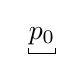
\begin{tikzpicture}[baseline=(term.base)]\node[inner sep=0pt] (term) {$p_0$};\draw ([yshift=-1pt]term.south west) -- ([yshift=-3pt]term.south west) -- ([yshift=-3pt]term.south east) -- ([yshift=-1pt]term.south east);\end{tikzpicture}=\underset{\sigma}{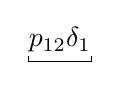
\begin{tikzpicture}[baseline=(term.base)]\node[inner sep=0pt] (term) {$p_{12}\delta_1$};\draw ([yshift=-1pt]term.south west) -- ([yshift=-3pt]term.south west) -- ([yshift=-3pt]term.south east) -- ([yshift=-1pt]term.south east);\end{tikzpicture}}=\underset{\mathrm{id}}{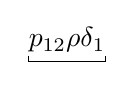
\begin{tikzpicture}[baseline=(term.base)]\node[inner sep=0pt] (term) {$p_{12}\rho\delta_1$};\draw ([yshift=-1pt]term.south west) -- ([yshift=-3pt]term.south west) -- ([yshift=-3pt]term.south east) -- ([yshift=-1pt]term.south east);\end{tikzpicture}}=\underbrace{p_{12}\rho^2\delta_1}}\]
\[\deleted{(\underset{p_{23}}{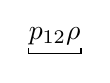
\begin{tikzpicture}[baseline=(term.base)]\node[inner sep=0pt] (term) {$p_{12}\rho$};\draw ([yshift=-1pt]term.south west) -- ([yshift=-3pt]term.south west) -- ([yshift=-3pt]term.south east) -- ([yshift=-1pt]term.south east);\end{tikzpicture}})\delta_1\overset{??}{\ne}\unsure{p_{22}|p_{12}|p_{23}}(\underset{\delta_2}{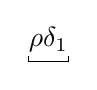
\begin{tikzpicture}[baseline=(term.base)]\node[inner sep=0pt] (term) {$\rho\delta_1$};\draw ([yshift=-1pt]term.south west) -- ([yshift=-3pt]term.south west) -- ([yshift=-3pt]term.south east) -- ([yshift=-1pt]term.south east);\end{tikzpicture}})}\]
\[\boxed{\begin{aligned}
\delta_0p_0&=p_{12}\overset{\delta_3}{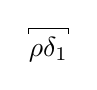
\begin{tikzpicture}[baseline=(term.base)]\node[inner sep=0pt] (term) {$\rho\delta_1$};\draw ([yshift=1pt]term.north west) -- ([yshift=3pt]term.north west) -- ([yshift=3pt]term.north east) -- ([yshift=1pt]term.north east);\end{tikzpicture}}\\
\mathrm{id}_{E_1}&=p_{12}\underset{\delta_2}{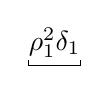
\begin{tikzpicture}[baseline=(term.base)]\node[inner sep=0pt] (term) {$\rho_{\deleted{\unsure{1}}}^{2}\delta_1$};\draw ([yshift=-1pt]term.south west) -- ([yshift=-3pt]term.south west) -- ([yshift=-3pt]term.south east) -- ([yshift=-1pt]term.south east);\end{tikzpicture}}\\
\sigma&=p_{12}\delta_1
\end{aligned}}\]
\margin{$\boxed{\sigma_3\delta_1=\delta_1}$\\$\boxed{p_{12}\sigma_3=\sigma p_{12}}$}
\deleted{$\unsure{(\mathrm{Ens})|\mathrm{ens}}$}
\diagram{\begin{tikzcd}[ampersand replacement=\&,column sep=large,row sep=small,execute at end picture={\draw (current bounding box.north west) -- (current bounding box.north east) -- ([yshift=10pt]current bounding box.south east);\draw ([yshift=4pt]current bounding box.south east) -- (current bounding box.south east) -- (current bounding box.south west) -- ([yshift=-4pt]current bounding box.north west);}]
\deleted{\unsure{\mathcal G|\mathfrak S}_{\unsure{2|1}}}\&\mathcal G_2\&\mathcal G_3\\
E_0\arrow[r,bend right=30,"\delta_0"']\&E_1\arrow[l,"p_0"']\arrow[r,bend right=30,"\delta_1"']\&E_2\arrow[l,"p_{12}"']
\end{tikzcd}}
\[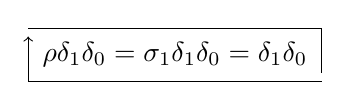
\begin{tikzpicture}[baseline=(eq.base)]\node[inner sep=5pt] (eq) {$\rho\delta_1\delta_0=\sigma_1\delta_1\delta_0=\delta_1\delta_0$};\draw (eq.north west) -- (eq.north east) -- ([yshift=3pt]eq.south east);\draw (eq.south east) -- (eq.south west);\draw[->] (eq.south west) -- ([yshift=-3pt]eq.north west);\end{tikzpicture}\]
\[\underset{p_{\unsure{2|1}}}{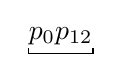
\begin{tikzpicture}[baseline=(term.base)]\node[inner sep=0pt] (term) {$p_0p_{12}$};\draw ([yshift=-1pt]term.south west) -- ([yshift=-3pt]term.south west) -- ([yshift=-3pt]term.south east) -- ([yshift=-1pt]term.south east);\end{tikzpicture}}\unsure{=|\ne}p_0\overset{p_{12}}{\begin{tikzpicture}[baseline=(term.base)]\node[inner sep=0pt] (term) {$\underset{p_{31}}{\begin{tikzpicture}[baseline=(term.base)]\node[inner sep=0pt] (term) {$p_{12}\deleted{\unsure{\sigma}}\rho^2$};\draw ([yshift=-1pt]term.south west) -- ([yshift=-3pt]term.south west) -- ([yshift=-3pt]term.south east) -- ([yshift=-1pt]term.south east);\end{tikzpicture}}\sigma_2$};\draw ([yshift=1pt]term.north west) -- ([yshift=3pt]term.north west) -- ([yshift=3pt]term.north east) -- ([yshift=1pt]term.north east);\end{tikzpicture}}\]
\margin{2}
